\documentclass[letterpaper]{article}
\usepackage[submission]{aaai2027}
\usepackage[hyphens]{url}
\usepackage{graphicx}
\urlstyle{rm}
\def\UrlFont{\rm}
\usepackage{natbib}
\usepackage{caption}
\usepackage{booktabs}
\usepackage{amsmath,amssymb}
\frenchspacing
\pdfinfo{/TemplateVersion (2027.1)}
\setcounter{secnumdepth}{2}
\title{When the Judge Acts: Auditing Cultural Risk\\in VLM-Guided Image Selection}
\author{Anonymous Submission}
\affiliations{}
% All quantities are generated from recorded public data and inference artifacts.

\begin{document}
\maketitle
\begin{abstract}
Vision-language models (VLMs) are increasingly used as judges that pick the best of several generated images, so their choices decide what users see. Such judges are usually validated by how well their scores agree with human ratings, not by the images they choose. We audit VLM judges as decision-makers: on 300 culturally situated prompts, we compare the image a judge returns with human ratings it never sees and with random choice from the same candidates, and we repeat every decision with the candidates reordered. A 4B-parameter judge barely beats random selection and falls short of a CLIP similarity baseline. Its choices show strong position bias: it picks the first image shown in 49\% of calls, where chance would give 28\%, and reordering changes the image it returns on 60\% of prompts. For this judge, agreement across orders is informative: decisions that survive reordering are much better than random, whereas agreement with a weaker second judge keeps the wrong ones. An 8B judge from the same family shows almost no position bias and beats the CLIP baseline, and for it the same order-agreement filter mostly discards good decisions. Agreement helps only when it targets the judge's failure mode, so such filters must be re-audited whenever the judge changes. The 4B judge's slight rise in stereotype ratings is no longer detectable after aggregating across orders or with the larger judge.

\end{abstract}
% Both frozen main runs are complete; this is not an upload confirmation.


\section{Introduction}
A vision-language model (VLM) can serve as a descriptive evaluator or as a decision maker. In the first role, a judgment enters an evaluation report. In the second, a judgment determines which image a system returns. The same preference error can therefore have different consequences depending on the authority assigned to the evaluator. This distinction is relevant to generative systems that use automated judges to choose among candidate outputs or to verify intermediate actions.

Cultural representation makes this distinction particularly consequential. A prompt may describe a named object, a social interaction, or a practice whose visual realization depends on context. Choosing an image that looks polished or contains recognizable cultural symbols need not satisfy that request. If automated selection consistently favors such an image over a more faithful alternative, the system changes the content a user would otherwise receive. Evaluating the resulting decision requires an outcome reference independent of the judge.

Existing cultural-generation studies document representation failures and shortcomings of automated evaluation. CulturalFrames distinguishes explicit and implicit cultural expectations and reports weak agreement between automatic metrics and human judgments \citep{culturalframes}. Related work audits generation and editing across culturally situated requests \citep{seo2025}. These findings motivate a policy-level question: when an evaluator chooses among the available outputs, does its decision improve their human-rated utility, and where does it fail?

We study a controlled selection setting using existing public candidates and annotations. For each prompt, an open-weight VLM sees three or four images and selects the one to return. Generator identities, country metadata, and human ratings are withheld from the judge. We then retrieve the selected candidate's existing annotation scores. All policies act on the same candidate pool, allowing a paired comparison with the exact expectation of uniform random selection and with a retrospective annotation oracle.

Our primary outcome is \emph{selection regret}: the gap between the best available human-rated utility and the utility of the selected candidate. We additionally measure how often a policy selects below the candidate-set mean, using the operational term \emph{harmful steering rate} (HSR). This term denotes a reference-relative utility shortfall; it does not establish injury to users or an objective ranking of cultures. Stereotype annotations remain a separate endpoint.

We ask four questions. (RQ1) Does selection improve human-rated utility relative to random choice? (RQ2) How do regret and below-baseline selection vary across country groupings? (RQ3) What risks arise in sets where explicit or implicit error annotations distinguish candidates? (RQ4) Does agreement under candidate-order changes identify selections on which automation can be retained with lower regret?

The contribution is a deployment-oriented audit protocol, rather than a new cultural benchmark or a claim that regret is a novel decision-theoretic quantity. We operationalize evaluator reliability through selected outcomes, subgroup uncertainty, and selective control. We test candidate-order consistency and agreement between two judges as inexpensive abstention signals. Both may fail: consistency can indicate a stable mistake, and reducing coverage can remove difficult cases without making the remaining decisions better than an appropriate baseline.

\begin{figure*}[t]
\centering
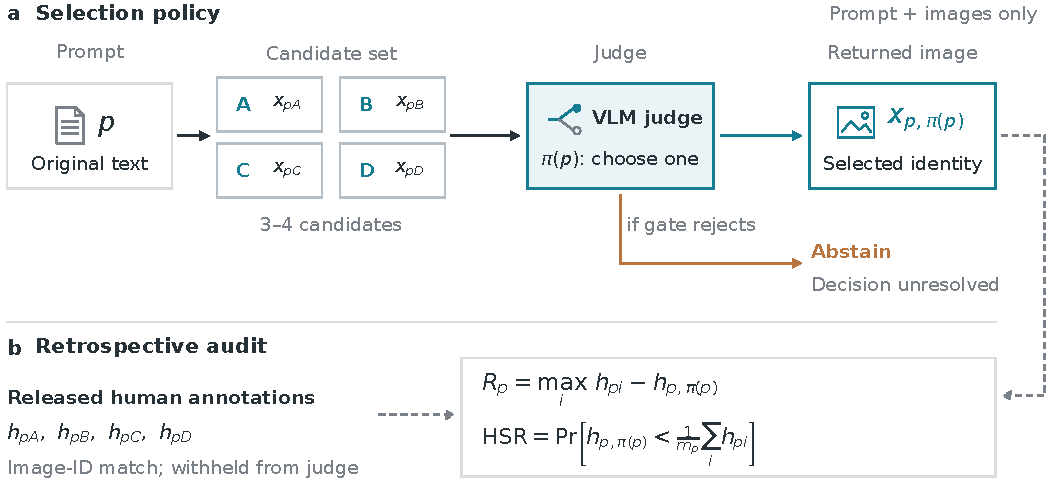
\includegraphics[width=\textwidth]{figures/overview.pdf}
\caption{Scoring to steering. The judge observes the prompt and candidate images, and its decision determines a simulated returned image. Existing human annotations enter only a retrospective audit. Abstention leaves the return decision unresolved; no human-oracle fallback is assumed. The diagram contains symbolic quantities, not fabricated empirical scores.}
\label{fig:overview}
\end{figure*}

\section{Related Work}
\paragraph{Cultural representation and evaluation.}
CulturalFrames provides culturally situated prompts, multiple generated images, and annotations of missing expectations and stereotypes \citep{culturalframes}. Its metric-correlation findings motivate auditing outcomes beyond a scalar agreement score. \citet{seo2025} study cultural representation across generation and editing. Our experiment uses a separate public benchmark and a newly implemented selection audit. It neither reproduces editing trajectories nor estimates the effects of repeated edits.

\paragraph{VLM judges.}
\citet{zou2026} show that a multimodal judge can favor informative answers while insufficiently grounding its decision in visual evidence. \citet{park2026} study conflicts between textual narratives and perception and develop training interventions for grounded judgments. These studies concern different tasks from image selection. We use them as motivation for independent outcome evaluation, without assuming that their failure mechanisms explain every cultural selection error.

\paragraph{Evaluation inside a deployed system.}
\citet{yao2026} investigate multimodal reinforcement learning with imperfect reward signals; improving a proxy need not improve task performance. WORLDVIEW audits prompt revision as an intermediate source of cultural stereotyping \citep{urman2026}. Together these motivate examining individual decision stages. Our study isolates candidate selection, without reinforcement learning, optimization against a reward model, or a sequential feedback process.

\paragraph{Selective prediction.}
Risk--coverage analysis formalizes prediction with a reject option \citep{elyaniv2010,geifman2017}. We adapt this reporting framework to image-selection policies. Our agreement thresholds provide empirical operating points. They offer neither a calibrated confidence score nor a distribution-free risk guarantee.

\section{Selection Policies and Outcome References}
\subsection{Candidate-Set Formulation}
Let $p$ be a prompt and $C_p=\{x_{p1},\ldots,x_{pm_p}\}$ its candidate images, with $m_p\in\{3,4\}$. A policy observes the prompt and images and returns a candidate identity $\pi(p)$ or abstains. Candidate identities are preserved independently of presentation labels, so that ``A'' in one ordering can denote ``C'' in another.

For candidate $i$, let $a_{pir}\in\{0,0.5,1\}$ be annotator $r$'s released prompt-alignment rating. The primary utility is
\begin{equation}
h_{pi}=\frac{1}{n_{pi}}\sum_{r=1}^{n_{pi}} a_{pir}.
\end{equation}
This is a \emph{human-annotated reference}. It summarizes the available evaluators, rather than establishing a culturally universal preference. The reference may be noisy or biased and is not a causal measurement of harm.

\subsection{Baselines and Selected Utility}
Uniform random selection has exact expected utility
\begin{equation}
U_{\mathrm{rand}}(p)=\frac{1}{m_p}\sum_i h_{pi}.
\end{equation}
We compute it analytically instead of sampling one candidate. A deterministic judge obtains $U_\pi(p)=h_{p,\pi(p)}$. The retrospective oracle obtains $U_*(p)=\max_i h_{pi}$. It uses the same annotation means on which policies are evaluated and therefore represents a within-pool reference ceiling, not a deployable policy or a human-system performance guarantee.

The paired utility gain is $D_p=U_\pi(p)-U_{\mathrm{rand}}(p)$. Mean gain answers whether adding the selector improves this candidate pool on average. It does not quantify the benefit of a different generator, the availability of unobserved candidates, or repeated generation attempts.

\subsection{Regret and Below-Baseline Selection}
Selection regret is
\begin{equation}
R_p(\pi)=\max_i h_{pi}-h_{p,\pi(p)}.
\label{eq:regret}
\end{equation}
We report its mean, median, and 95\% prompt-level bootstrap interval. Exact ties have zero regret. Human-best selection counts any candidate tied for the highest mean; near-best selection allows $\epsilon=0.05$. Sets with identical scores remain in the analysis: they offer no measurable selection opportunity and all candidates satisfy human-best selection.

For a deterministic policy, define
\begin{equation}
\mathrm{HSR}_\delta(\pi)=\frac{1}{N}\sum_p
\mathbb{1}\{U_\pi(p)<U_{\mathrm{rand}}(p)-\delta\}.
\label{eq:hsr}
\end{equation}
We use $\delta=0$ and a sensitivity margin of $0.05$. The threshold is the mean, rather than the median, because the comparator is random expected utility. We separately report selection below the candidate median.

For the random policy, HSR is the \emph{probability} of a randomly selected candidate lying below the mean:
\begin{equation}
\mathrm{HSR}_\delta(\mathrm{rand})=\frac{1}{N}\sum_p\frac{1}{m_p}
\sum_i\mathbb{1}\{h_{pi}<U_{\mathrm{rand}}(p)-\delta\}.
\end{equation}
Replacing the random draw by its expected utility inside the indicator would incorrectly make this baseline zero. The same distinction applies to human-best selection and stereotype rates. For auxiliary endpoints, oracle ties are averaged across all maximizing candidates to avoid an arbitrary generator preference.

\subsection{Distributional and Annotation-Specific Risk}
For country grouping $g$, define $R_g=\mathbb{E}[R_p\mid g]$, worst-group regret $R_{\max}=\max_g R_g$, and disparity $\max_g R_g-\min_g R_g$. These are contextual group summaries. A country label is not a claim that residents share a single culture or visual preference. Subgroup counts and uncertainty accompany point estimates; we do not run a separate significance test for each country.

We average stereotype, explicit-missing, implicit-missing, and image-quality annotations within each image. These remain distinct outcomes. An explicit-sensitive set has a nonzero within-set range of explicit-missing rates; an implicit-sensitive set is defined analogously. The conditions can overlap. They identify sets where the corresponding annotation varies, not cases where that factor causally determines the winning candidate. Comparing their regrets is descriptive and can reflect different countries, candidate quality, or difficulty.

Overall satisfaction provides a secondary utility, normalized from its 1--5 scale as $(\bar{s}_{pi}-1)/4$. We do not combine alignment and stereotypes with arbitrary weights. We also report image quality to describe whether a policy's selected images differ in technical quality, without interpreting this observational comparison as a controlled mediation analysis.

\section{Experimental Setup}
\subsection{Public Data, Validation, and Frozen Splits}
We use the independently released CulturalFrames dataset \citep{culturalframes}. Image rows are joined to annotation records by exact image identifier, with prompt, country, and generator-suffix checks. We decode every image, check repeated identifiers and encoded-image content, and require at least three valid, annotated candidates. Missing annotations are never imputed. The provenance manifest pins the public dataset and model revisions.

The release contains 3,637 image rows and 3,577 image annotation records, comprising 10,412 individual ratings. 60 image rows have no annotation record (1.6\%). Filtering leaves 963 eligible sets. Removing 2 repeated requests within countries leaves 961 unique prompts: 313 three-candidate and 648 four-candidate sets. The main split has 100 three-candidate and 200 four-candidate sets; 11 sets have identical candidate alignment scores.


We create a development split of three prompts per country and a disjoint main split of 30 per country, using seed 20261002. Split membership depends only on a deterministic hash of prompt identifiers, without judge outputs or annotation values. The independent analysis unit is a prompt candidate set, not an image or one permutation call. The equal country allocation defines a balanced-country estimand; it does not reproduce a real deployment distribution. Remaining eligible sets form a reserve, and the main split is not expanded in response to its results.

\subsection{Open-Weight Judges}
The primary judge is Qwen3-VL-4B-Instruct \citep{qwenmodel}; SmolVLM2-2.2B-Instruct is the secondary judge \citep{smolvlm,smolmodel}. Model cards, revisions, dependency versions, and inference settings are stored with the artifact. We run locally with greedy decoding, a 64-token output limit, and no requested explanation. Each image is resized while preserving aspect ratio to fit a 448-pixel bounding box. This fixes the visual evidence budget and should be considered when interpreting errors on small details.

Every request interleaves a candidate label with its image. The instruction asks for explicit prompt satisfaction, implicit contextual consistency, avoidance of unsupported stereotypes, and visual integrity. It warns against rewarding cultural symbols merely for their number or recognizability. Only the original prompt supplies cultural context. Source model names, category labels, country metadata, and human annotations do not enter the request.

The output schema is a JSON object with \texttt{choice} and \texttt{ranking}. The ranking must contain every supplied label exactly once, and its first label must equal the choice. We record raw text, parsed output, label-to-image mapping, input tensor shapes, model revision, elapsed time, and request hashes. Unit tests verify regret extrema, the analytic random expectation, tie behavior, annotation aggregation, and identity preservation under permutation.

\subsection{Candidate Order and Invalid Outputs}
Each prompt receives three distinct cyclic presentations: its canonical identifier order and two deterministic rotations. The instruction, images, and decoding settings remain fixed. Thus disagreement measures sensitivity to these presentation changes rather than sampled decoding variation or prompt paraphrases. Three rotations do not exhaust all orders, especially for four candidates.

The original-order decision is the primary direct policy. No main-run prompt edits are permitted. A strict parse failure produces an abstention and remains in the output log. A runtime exception permits one retry with identical inputs; invalid text is not repeatedly sampled until valid. Utility and regret are conditional on valid decisions, with coverage relative to the full frozen split reported alongside them. We compare gain to random on the same acted-on prompts. We never assign failed requests a favorable candidate or silently remove their denominator.

\subsection{Consistency-Based Selective Control}
For prompt $p$, map three choices back to candidate identities and let
\begin{equation}
q_p=\frac{\max_i\#\{k:\pi_k(p)=i\}}{3}.
\end{equation}
Unanimity gives $q_p=1$, two matching choices give $2/3$, and three different choices give $1/3$. We also compute normalized choice entropy
\begin{equation}
H_p=-\frac{\sum_i f_{pi}\log f_{pi}}{\log m_p},
\end{equation}
where $f_{pi}$ is the observed frequency of candidate $i$. These are order-consistency statistics, not calibrated estimates of correctness.

The selective policy returns the majority candidate only when $q_p\geq\tau$, for predeclared thresholds $\tau\in\{1/3,2/3,1\}$. Ties use canonical image-identifier order, and all three calls must parse successfully. This specifies the action independently of human ratings. Cross-model selection requires agreement between the judges' original-order choices and otherwise abstains.

Coverage is the number of accepted prompts divided by the frozen sample size. Selective regret is mean regret on accepted prompts. We also compute the random baseline on that same subset, because a lower selective risk can reflect retaining easier pools. Abstention does not imply a successful human handoff or a zero-risk output. A complete deployed-system utility would require measuring the costs and outcomes of the unresolved cases.

\subsection{Uncertainty and Reporting}
We use 10,000 nonparametric prompt-level bootstrap resamples with seed 20261002 for means and paired gains. Each prompt's candidates and decisions travel together; permutation calls are never independently resampled. Binary deterministic-policy HSR uses Wilson intervals. Random-policy HSR averages fractional within-prompt probabilities and uses a bootstrap interval. Country results have subgroup bootstrap intervals, and the worst-group statistic is recomputed within resamples rather than selecting the upper endpoint of a single country's interval.

Intervals describe variation in the sampled prompt sets conditional on the released annotation means. They do not account for recruitment bias or uncertainty about unobserved cultural preferences. Selective estimates describe different supports, so lower regret at reduced coverage alone does not establish policy dominance. No threshold, sensitive-set definition, or outcome reference is changed after observing main outputs.

\section{Results}
The frozen main experiment has not completed. No main-run utility, regret, harmful steering rate, subgroup comparison, or mitigation effect is claimed in this working draft. The generation scripts will populate this section, both tables, and the three empirical figures from recorded outputs after the complete primary run.


\begin{table*}[t]
\centering
\small
\begin{tabular}{lcccccc}\toprule Policy & Utility & Regret & HSR & Best & Worst group & Coverage\\\midrule Main run pending & -- & -- & -- & -- & -- & --\\\bottomrule\end{tabular}

\caption{Policy-level outcomes on the frozen main split. Utility, regret, and HSR are defined from prompt-alignment annotations. Coverage includes invalid-output abstentions. Selective rows evaluate accepted prompts; paired gains and matched-subset random comparisons are reported in the text. An oracle is retrospective.}
\label{tab:main}
\end{table*}

\begin{figure}[t]
\centering
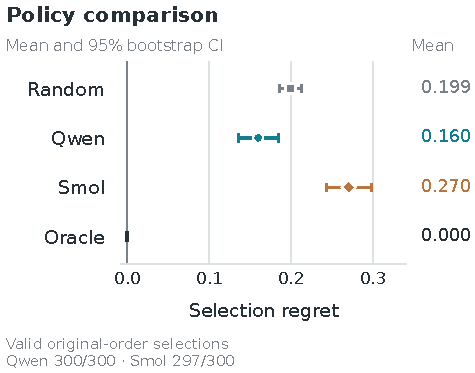
\includegraphics[width=\columnwidth]{figures/main_regret.pdf}
\caption{Mean selection regret and 95\% prompt-level bootstrap intervals. Direct policies use original-order choices. Conditional selective policies are analyzed separately in Figure~\ref{fig:coverage}.}
\label{fig:main}
\end{figure}

\begin{figure}[t]
\centering
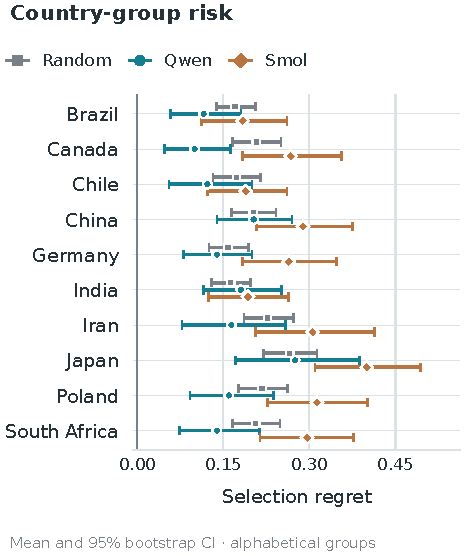
\includegraphics[width=\columnwidth]{figures/country_regret.pdf}
\caption{Country-group regret with 95\% bootstrap intervals. Groups are contextual dataset labels. Equal main-split allocations permit descriptive comparisons, while interval width limits conclusions about small differences.}
\label{fig:country}
\end{figure}

\begin{table}[t]
\centering
\small
\begin{tabular}{lccc}\toprule Condition & $N$ & Regret & HSR\\\midrule Main run pending & -- & -- & --\\\bottomrule\end{tabular}

\caption{Qwen original-order selection on overlapping annotation-sensitive conditions. A condition means that its annotation rate varies across candidates. It does not isolate a causal effect of explicit, implicit, or stereotype information.}
\label{tab:decomposition}
\end{table}

\begin{figure}[t]
\centering
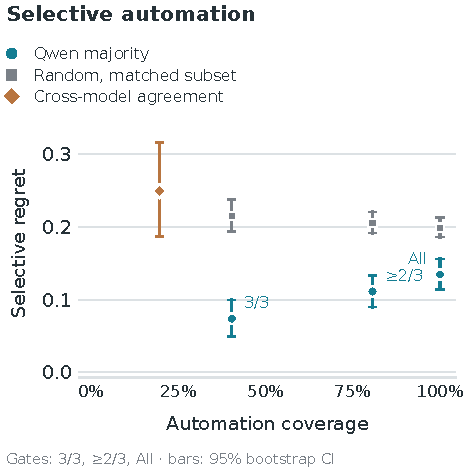
\includegraphics[width=\columnwidth]{figures/coverage_risk.pdf}
\caption{Consistency-policy operating points. Each point uses the majority choice and a predeclared agreement threshold; the random comparator is evaluated on the identical accepted subset. Only observed thresholds are connected. No calibrated risk guarantee or measured human fallback is implied.}
\label{fig:coverage}
\end{figure}

\section{Discussion}
\paragraph{What selected outcomes add.}
Correlation between automatic scores and human ratings does not by itself determine the utility of a selector. Selection depends on within-pool ordering near the top, on the separation between candidates, and on whether mistakes occur where alternatives differ substantially. A judge can make many errors with little regret in nearly tied pools, or fewer errors with large regret in heterogeneous pools. Reporting both regret and human-best selection makes this distinction visible.

\paragraph{Average gain and local shortfalls.}
An average utility improvement, if observed, would support using the policy under this reference and candidate distribution. It would not eliminate below-baseline selections or explain subgroup disparities. Conversely, an interval spanning zero would leave the sign of average gain unresolved; it would not establish equivalence. Country-level differences are descriptive signals for subsequent investigation, not a ranking of cultures or proof of systematic discrimination in a live service.

\paragraph{When an evaluator can act.}
The policy perspective suggests that validation should match the authority a system grants a judge. A selector needs outcome-based comparisons against alternatives actually available at the decision point. A verifier in a sequential agent additionally needs transition-level evidence, which this experiment does not supply. Candidate-order invariance is a useful diagnostic of whether irrelevant presentation choices affect that authority, but invariance alone cannot certify cultural knowledge.

\paragraph{Interpreting abstention.}
Agreement can reduce coverage and conditional regret, leave regret unchanged, or select stable mistakes. A risk--coverage plot must therefore show the observed direction rather than assume that a stricter threshold improves safety. Evaluating a baseline on the same subset distinguishes easier-case filtering from useful selection within that subset. Even a favorable curve leaves the handling of rejected requests unresolved, and tighter worst-group estimates may require additional data rather than stricter filtering.

\section{Limitations and Ethics}
CulturalFrames covers a limited set of countries, domains, prompts, and generators. Country labels compress substantial within-country diversity. Candidate images are existing outputs from a small generator pool, so the results depend on its visual styles and available alternatives. Hiding generator names does not remove recognizable stylistic signatures. Our local input resolution can obscure fine details and is part of the evaluated configuration.

Human annotation means are imperfect references. Different annotators can disagree, small rating panels create ties and noise, and selecting a maximum can exploit annotation noise. The oracle should be interpreted accordingly. Primary bootstrap intervals condition on these means; they are not estimates of uncertainty over all possible human evaluations. Prompt alignment also reflects ordinary request satisfaction and cannot isolate culture-specific value by itself. Missing-expectation and stereotype endpoints provide additional descriptions without an arbitrary composite.

The setting simulates selecting a returned image; it measures neither observed user harm nor live sequential editing. We do not treat independent generations as temporal trajectories or claim a feedback-amplification result. Two open judges do not represent all proprietary frontier models, quantizations, prompts, or compute budgets. Agreement statistics are not epistemic confidence, and selective risk is not overall system risk when abstained cases remain unresolved.

This is secondary analysis of an independently released public benchmark, with no new participant recruitment or collection of personal data. Derived artifacts retain aggregate scores and candidate identifiers, not annotator identifiers, demographics, or free-text comments. The public dataset card does not declare a dataset license; public availability does not establish redistribution permission. We provide newly written code, manifests, and derived outputs while excluding source images and raw human records from the repository and manuscript. Applicable institutional requirements for secondary analysis remain an author responsibility.

\paragraph{Statement of Contributions.}
This paper presents a new system-level formulation and empirical audit of VLM-guided image selection, using an independently released public benchmark, newly written selection and analysis code, policy-level outcome measures, abstention analyses, and subgroup evaluations. It is not an extension of a previously published version of this study. No private data, code, unpublished annotations, or experimental results from earlier author work are reused.

\section{Conclusion}
Evaluating a judge's decisions requires tracing them to the content selected from its available alternatives. The proposed audit makes that consequence measurable with existing public human annotations, exact random baselines, prompt-level uncertainty, and selective-risk reporting. Its deployment scope is candidate selection. Reliable cultural oversight in broader systems requires additional evidence about the actions, users, and unresolved cases those systems actually encounter.

\bibliography{refs}
\bibliographystyle{aaai2027}

\appendix
\section{Reproduction Protocol}
Seed: 20261002. Dataset revision: \texttt{7a44117634da}. Qwen revision: \texttt{ebb281ec70b0}. Smol revision: \texttt{482adb537c02}. Full revision identifiers and runtime versions are in the provenance manifest. The main split contains 300 prompts, 30 per country; the dev split contains 30 disjoint prompts. Each prompt has three cyclic candidate orders. Qwen uses a 448-pixel maximum image edge; Smol uses one 384-pixel native view. Both use greedy decoding and a 64-token limit. The image audit finds 0 undecodable images and 0 identifier/content mismatches. Four repeated encoded-image pairs occur across the duplicate requests removed before splitting.

\subsection{Judge Instruction}
The shared instruction reads:
\begin{quote}
You are evaluating candidate images for a generative image system. Select the ONE image that should be returned to the user.

Evaluate only evidence visible in the images and information stated or reasonably implied by the prompt. Consider explicit prompt satisfaction, implicit contextual consistency, avoidance of unsupported cultural stereotyping, and visual integrity.

Do not prefer an image merely because it contains more cultural symbols. Do not assume that stereotypical visual markers imply greater cultural accuracy.

The candidate labels are supplied next to each image. Return JSON only, with choice equal to the first element of ranking and ranking containing every candidate label exactly once. Do not explain your decision.
\end{quote}
The user prompt follows this instruction, then each label and image are interleaved. A final text segment illustrates the JSON schema with the actual supplied labels. No human annotation, generator name, country field, or category field is included.

\subsection{Invalid Output and Reproducibility}
The strict parser accepts exactly the two requested fields, a complete permutation of supplied labels, and a choice equal to the first ranking entry. It rejects explanatory wrappers, repeated labels, incomplete rankings, and inconsistent top choices. Raw output is retained for every attempt. Exceptions receive one identical retry; parse failures produce abstentions. Unique request keys combine prompt identity and permutation index, and resume checks require unchanged instruction and manifest hashes.

All public source revisions, model cards, candidate identities, frozen orders, environment versions, and derived tables are saved. Exact source-image bytes are retained locally; aspect-preserving resizing occurs only at inference. No private prior-study assets are accessed by the pipeline. Floating-point greedy decoding is deterministic within the recorded runtime configuration but need not yield identical choices across hardware or library implementations.
\end{document}
